\section{Historia contemporánea y usos.} \label{now-history}

Menos de una hora después de que Hofmann se administrase la dosis, estaba claro que el LSD era el culpable de su anómalo estado. Ayudado por su asistente, regresó en bicicleta a casa atravesando un paisaje ondulante. Tumbado en el sofá, su alrededor se tornaba grotesco. Su vecina que traía leche se convirtió en una malvada bruja. Estaba aterrorizado de que su experimento dejase a una familia sin padre, mas cuando llegó el médico, este no aconsejó más que dejar pasar el tiempo, pues sus constantes vitales eran correctas. Gran acierto, ya que de aquél escenario macabro descendió a la realidad, pudiendo disfrutar del residuo de sinestesias e imágenes caleidoscópicas. Al día siguiente se encontraba con la cabeza totalmente fresca, pudiendo recordar toda su experiencia.

Hofmann visionó en el LSD una droga de enormísima utilidad en farmacología, neurología y particularmente en psiquiatría. Jamás habría podido anticipar sin embargo que fuese a ser utilizada de manera recreativa después de lo vivido.

Tras informar a su supervisor, el departamento farmacológico de Sandoz se puso manos a la obra a estudiar la tolerancia y toxicidad de la sustancia. Los primeros exámenes en animales mostraban a gatos que observaban a la nada y en lugar de atacar a ratones, los miraban horrorizados. Las arañas construían telas más eficientes en dosis bajas pero rudimentarias en dosis altas. Al introducirse en una comunidad de chimpancés, incluso si solo unos pocos individuos lo tomaban, el grupo entero entraba en conflicto debido a que estos no seguían las leyes jerárquicas de su tribu.

Demostrada la seguridad del LSD y probado sistemáticamente en humanos, Sandoz lo comercializó como un fármaco experimental: el \textit{Delysid}. Entre sus usos se citaba además la autoexperimentación del psiquiatra para ganar perspectiva sobre la emoción interna de sus pacientes, pues la experiencia servía como modelo de distintas afecciones.

\subsection{Terapia psicodélica, arte y recreación, prohibición.}

El LSD no actúa como un medicamento \textit{per se}, es decir, no arregla --- que sepamos --- ningún desequilibrio químico como sí lo hace un antidepresivo. Sin embargo, dados los peculiares efectos que produce sobre la consciencia, sus usos como fármaco auxiliar en psicoterapia y psicoanálisis han sido muy abundantes. Al llevar al extremo el estado interno del usuario y hacer que reaparezcan recuerdos olvidados (en forma de \enquote{reviviscencia}), el LSD es una herramienta útil para liberar material reprimido, haciéndolo eficiente para tratar el trauma. Además, al disolver la barrera entre el tú y el yo, facilita el desprendimiento de problemas centrados en el ego. También se ha utilizado en pacientes terminales de cáncer que desarrollan mucha tolerancia a los analgésicos, aunque esto plantea cuestiones éticas. La experiencia de disociación corporal impide que el dolor penetre en la consciencia y facilita el coraje para afrontar la propia muerte. Este uso requiere supervisión y una preparación especial, a menudo siendo útil que un psicoterapeuta o una figura religiosa guíe la experiencia. El célebre escritor Aldous Huxley pidió en su lecho de muerte a su mujer ser inyectado con 100 microgramos, varias dosis si fuese necesario.

A principios de los 60 el LSD se extiende como la pólvora por occidente, con una influencia particular sobre la sociedad estadounidense que se ve acompañada casual o causalmente por el nacimiento del movimiento hippie. El doctor Timothy Leary de la universidad de Harvard fue una figura muy relevante en la difusión de LSD en los Estados Unidos. Realizó exámenes sobre su uso en miembros del clero, convictos y artistas, aunque sus obras rápidamente perdieron el carácter científico y fue expulsado de la universidad. Convertido al hinduísmo, pasó a ser uno de los principales líderes del movimiento hippie. Con el grito estampado hasta la saciedad de \enquote{Turn on, tune in, drop out}, alentaba a la juventud a consumir LSD (\textit{turn on}) para explorar su mundo interior (\textit{tune in}) y finalmente desprenderse de la vida burguesa, los estudios, el trabajo y toda cadena con el cántico \enquote{\textit{drop out}} (Figura \ref{albums}).

\begin{figure}[H]
	\centering
	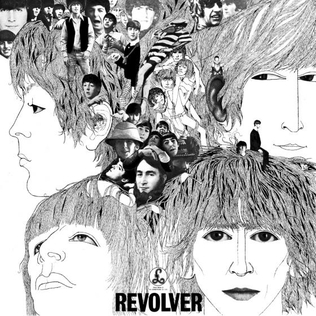
\includegraphics[height=.2\textheight]{media/10-revolver.jpg}
	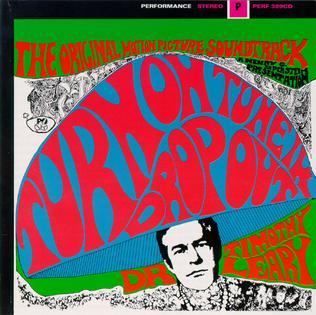
\includegraphics[height=.2\textheight]{media/10-leary.jpg}
	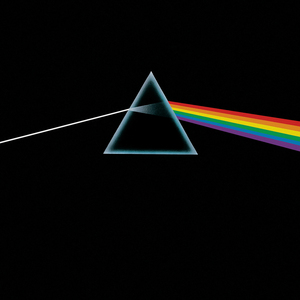
\includegraphics[height=.2\textheight]{media/10-dsotm.png}
	\caption{Carátulas de los álbumes \textit{Revolver} (The Beatles), \textit{Turn On, Tune In, Drop Out} (Timothy Leary) y \textit{The Dark Side of the Moon} (Pink Floyd), muy influídos por el LSD.}
	\label{albums}
\end{figure}

Esta subversión de las estructuras convencionales era un pronunciamiento abierto que desafiaba --- recordando a los chimpancés que perdieron su estructura jerárquica --- a toda autoridad social y política. El Dr. Leary fue arrestado en Kabul y encarcelado por posesión de drogas. En 1976, ya libre, se mantuvo ocupado con cuestiones como la relación entre el SNC y el espacio interestelar.

El LSD siguió una ruta histórica similar a la de la mescalina: comenzó como un compuesto químico de interés en agrupaciones científicas y psiquiátricas y se inmiscuyó entre intelectuales. Las experiencias estéticas e introspectivas inducidas lideraban el proceso creativo de los artistas, y de sus numerosas obras nació el arte psicodélico, que comprende toda creación realizada tras el uso de LSD y otros psicotrópicos como la mescalina o la psilocibina. El libro \textit{Psychedelic art} contiene una recopilación excelente de este género.

En la música, grupos tan populares como los Beatles fueron marcados por esta sustancia. Discos como \textit{Revolver}, o \textit{Sgt. Pepper’s Lonely Hearts Club Band} y canciones como \textit{Lucy in the Sky with Diamonds} (título que hoy sirve de alias a esta droga) recibieron una influencia estética propia del LSD. En conjunto, bandas coetáneas como Pink Floyd, Jefferson Airplane y The Grateful Dead concibieron el género del \textit{rock psicodélico}.

El LSD se introdujo también en las clases populares. Hofmann había previsto curiosidad por parte de los artistas e intelectuales, pero jamás pensó que su creación fuese a ser empleada como un embriagador común, y este uso provocó varios incidentes. Los experimentos clínicos y universitarios con la droga pasaron de ser compartidos en publicaciones científicas a ser presentados delante de todo el mundo en revistas y periódicos, donde las conclusiones eran exageradas. Los reportajes acerca de esta droga ya no se daban en tercera persona, sino que los mismos periodistas la consumían y relataban posteriormente sus experiencias. En los mercados estadounidenses aparecían libros relatando los efectos del LSD, muchas veces exaltándolos.

Toda esta literatura implantó en la cultura popular una idea falsa: que el solo uso de esta medicina era suficiente para lograr efectos milagrosos. Bajo semejante concepción, comenzó el imperio de la autoexperimentación. Los sesenta, con una crisis existencial de la sociedad estadounidense, la completa legalidad de la sustancia y la expiración de las patentes de Sandoz hicieron al LSD omnipresente. Como era de esperar, las experiencias populares se parecían más a las primeras de Albert Hofmann. \enquote{Malos viajes}, desorientación y pánico eran el producto habitual del experimento propio, a veces provocando accidentes y crímenes.

Entre 1964 y 1966 la polémica del LSD reinaba, con entusiastas diciendo que era una sustancia mágica y otros que señalaban los accidentes y crímenes que se cometían bajo sus efectos. Sandoz sufrió demandas masivas acerca de las propiedades de la sustancia. Finalmente en agosto de 1965 dejaron de producir y exportar públicamente el Delysid. A cambio, ofrecieron entregarlo a investigadores cualificados de todo el mundo, con asistencia tanto técnica como en muchos casos financiera. Sumado a una detallada descripción en el \textit{Catalogue of Literature on Delysid}, con la que se inhibió en buena medida el uso indebido.

Sandoz sin embargo no podía controlar todas las posibles excepciones. Las ideas erróneas en circulación y la total ausencia de legislación forzaron a Sandoz a cesar la producción de LSD y de alucinógenos similares como la psilocibina. A continuación siguió el \textit{Convenio sobre Sustancias Psicotrópicas} de la ONU y el establecimiento de estatutos como el \textit{Controlled Substances Act} en Estados Unidos, que no solo prohibía su posesión y distribución, sino que descartaba cualquier uso terapéutico de la sustancia. Su asociación a una \enquote{droga de la locura} disuadió a los psiquiatras de continuar empleándolo. El LSD, como condenado por una trágica maldición familiar, fue llevado al ostracismo al igual que su padre el ergot tres siglos antes.

El declive en uso de LSD ha afectado notablemente a su producción. En estudios psiquiátricos y neurobiológicos se ha visto sustituído por sustancias como la psilocibina encontrada en las setas alucinógenas, no solo por su semejanza en farmacología y efectos, sino porque su tiempo de acción más breve facilita su estudio. Como droga ilegal también se ha visto desplazado por derivados del cáñamo como el hachís y drogas sintéticas como la heroína y las anfetaminas, siendo habitualmente más tóxicos los sustitutos.

\subsection{Riesgos asociados al LSD.}

Actualmente la legislación no atribuye usos terapéuticos al LSD. Existen opiniones contrarias que argumentan que no hay peligro en el uso en entornos profesionales, algunas llegando a afirmar que el existente fuera de estos está relacionado con la clandestinidad y no con la sustancia. Es innegable que el uso de LSD está asociado a un conjunto de riesgos que deben ser conocidos tanto si se hace en un entorno profesional con supervisión médica como si no.

La desorientación intrínseca a todo experimento con LSD hace imposible descartar episodios de crisis, por más que se pueda minimizar mediante preparación. En los peores casos, la psicosis inhibirá la percepción de riesgo del individuo, produciendo accidentes fatales. En su defecto, una experiencia con visiones mortíferas puede conducir al suicidio. Aun si no son casos tan comunes, han de servir de advertencia. Frank Olson, un doctor estadounidense, consumió altas dosis de LSD sin su conocimiento. Se suicidó saltando por una ventana. Había sido víctima de experimentos farmacológicos del ejército estadounidense, y no fue hasta pasados 15 años que, con la revelación del proyecto MK Ultra, el director de la CIA William Colby y el presidente del gobierno Gerald Ford presentaron sus disculpas a la familia.

Es importante también analizar si el LSD es el fármaco óptimo para el bienestar del paciente, suministrándolo solo en los casos adecuados. Como el LSD intensifica el estado mental del momento, ofrecérselo a un paciente con la intención de curar un mal ánimo puede ser muy perjudicial. Tampoco debe ser utilizado sobre personalidades inestables, como aquéllas con tendencia a la psicosis. Esto incluye por lo general a la gente joven.

Es necesario un comentario acerca del uso personal que recibe el LSD. Existe un problema intrínseco al uso personal de cualquier droga. Si por definición estas actúan sobre el sistema nervioso afectando a la emoción y la percepción --- y nuestro juicio se basa precisamente en estas facultades --- entonces nuestra toma de decisiones se verá comprometida, incluyendo la propia decisión de consumir la droga. Ideas aceptadas o rechazadas en un estado de conciencia pueden no serlo en otro incluso a pesar de realizarse una planificación previa. Esta cuestión plantea un debate acerca de la relación del libre albedrío con el sistema nervioso, pero no lo trataremos.

Es imposible realizar un estudio científico acerca del uso personal de LSD, ya que de establecer un entorno controlado y realizar un seguimiento de cada individuo, el uso dejaría de ser personal. Dependemos entonces de la \enquote{sabiduría popular} relatada por periodistas y particulares como el propio Albert Hofmann. En diversas fuentes se habla por ejemplo del concepto de \textit{set y setting} como determinante para que los sentimientos durante una experiencia sean predominantemente positivos. Se denomina \textit{set} al conjunto de factores internos como el estado de ánimo previo y las expectativas, y \textit{setting} a los factores externos como el carácter del entorno, su iluminación, su ruido ambiente o las personas presentes. También se menciona la importancia de una persona de confianza como sustento emocional capaz de solicitar asistencia médica en caso de ser necesario. Se hace especial énfasis en la dosis, recomendándose empezar por unas muy bajas y llevar un registro con los efectos de cada una.

Finalmente es menester recordar que el LSD es ilegal, y que en consecuencia el mercado negro es la única vía de obtención. Esto plantea riesgos totalmente ajenos a los farmacológicos. Al no estar regulados, la pureza de los productos clandestinos es desconocida, y es común encontrarlos contaminados por otras sustancias. Además del problema de la pureza está el de la dosis: incluso si se adjunta la medida en microgramos (también llamados \enquote{\textit{gammas}}), esta puede estar alterada. Dada la abismal diferencia entre dosis de 25, 100 y 600 microgramos de LSD, la incertidumbre al momento de consumir un producto clandestino hace mucho más comunes las malas experiencias.

\newpage
